\section{Fonctionnalités}
\label{s:fonctionnalités}

\subsection{Image}
\subsubsection{Exportation d'image}
Il est possible d'exporter des rendus de la scène dans des fichiers PNG.
Pour ce faire, il suffit d'appuyer sur la barre espace et une capture d'écran de la fenêtre de l'application est sauvegardée dans le dossier \textit{/bin/data}.
Le fichier image est nommé en fonction de la date et de l'heure selon le format y$-$m$-$d\_hms.png.

\begin{figure}[H]
    \centering
	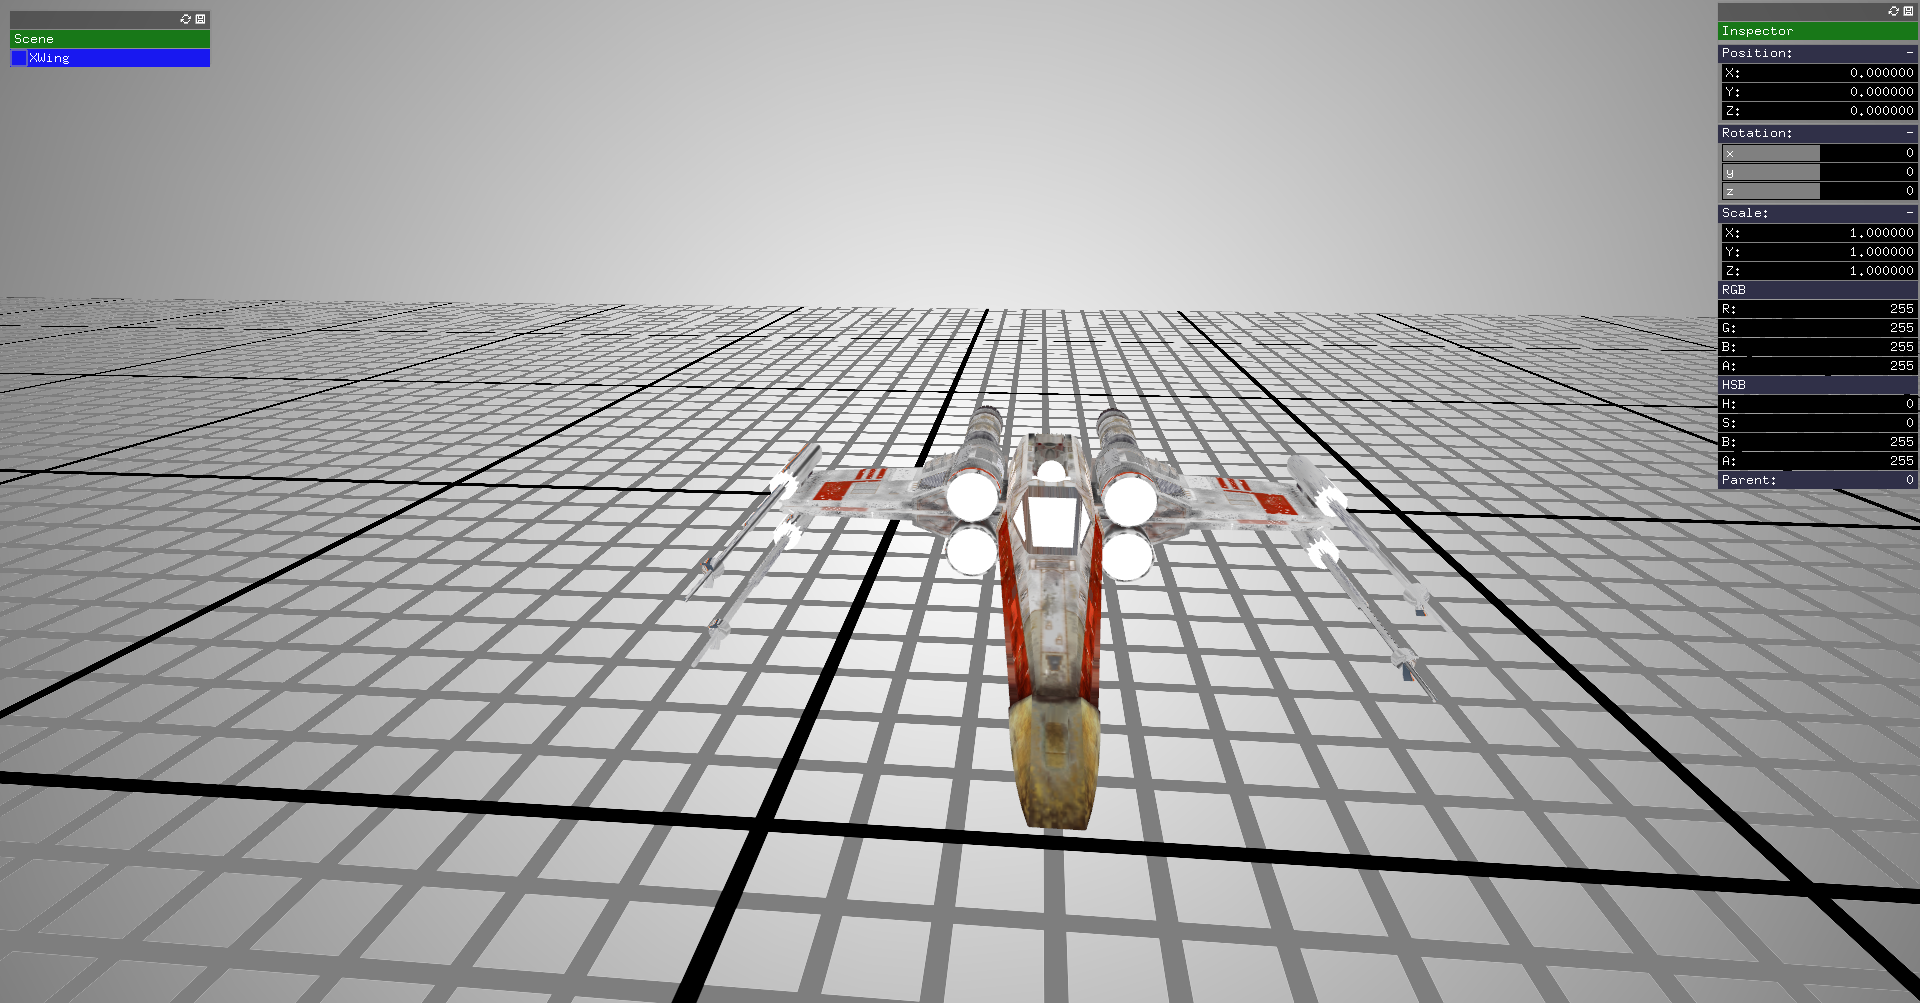
\includegraphics[scale=0.1]{fig/2018-3-11_22h34m38s.png}
	\caption{Exemple de capture d'écran}
	\label{fig:capture_ecran}
\end{figure}

\begin{figure}[H]
    \centering
	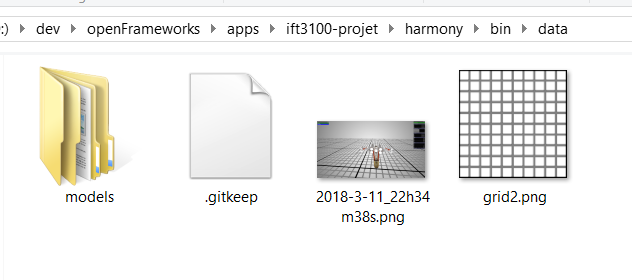
\includegraphics[scale=0.5]{fig/preuve-capture.png}
	\caption{Fichier exporté}
	\label{fig:preuve-capture}
\end{figure}

L'algorithme de capture d'écran est le suivant:
\begin{figure}[H]
    \centering
	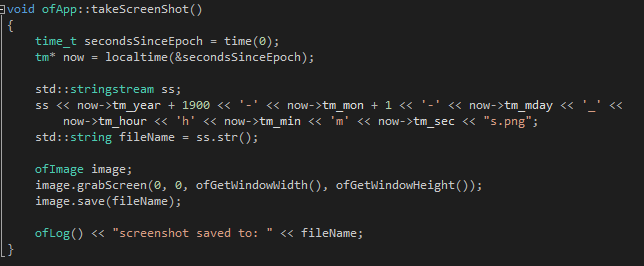
\includegraphics[scale=0.5]{fig/screenshotducodequiprenddesscreenshots.PNG}
	\caption{Code de la capture d'écran}
	\label{fig:capture_ecran}
\end{figure}

\subsubsection{Sélecteur de couleur}
\label{ss:selecteur_de_couleur}
L'inspecteur offre deux sélecteurs de couleurs affichant les valeurs des composantes de couleur de l'objet sélectionné et permettant de les modifier.
Chaque composante de couleur est encodée sur 8 bits, ce qui signifie que les sélecteurs acceptent des entiers entre 0 et 255.
\begin{figure}[H]
    \centering
	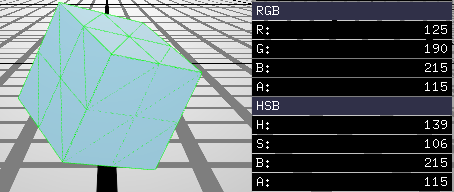
\includegraphics[scale=0.8]{fig/couleur.PNG}
	\caption{Sélecteurs de couleur}
	\label{fig:color_picker}
\end{figure}
Lorsque l'utilisateur entre une valeur dans un des champs, on récupère chacune des composantes et on applique cette couleurs à chaque vertex de l'objet sélectionné.

\subsubsection{Espace de couleur}
Un des sélecteurs de couleur de l'inspecteur permet de travailler en espace RGBA alors que l'autre permet de travailler en espace HSBA (voir la figure \ref{fig:color_picker}).
Lorsque la valeur d'une composante est modifiée dans un espace de couleur, l'autre sélecteur est mis à jour afin d'afficher les valeurs correspondantes.


\subsection{Dessin vectoriel}
\subsubsection{Primitives vectorielles}
Les primitives vectorielles offertes par cette application sont : une ligne, un triangle, un rectangle, un pentagone et un cercle.
Sur la figure suivante, on peut voir tous les objets qu'il est possible de créer dans l'application, incluant les primitives vectorielles.
\begin{figure}[H]
    \centering
	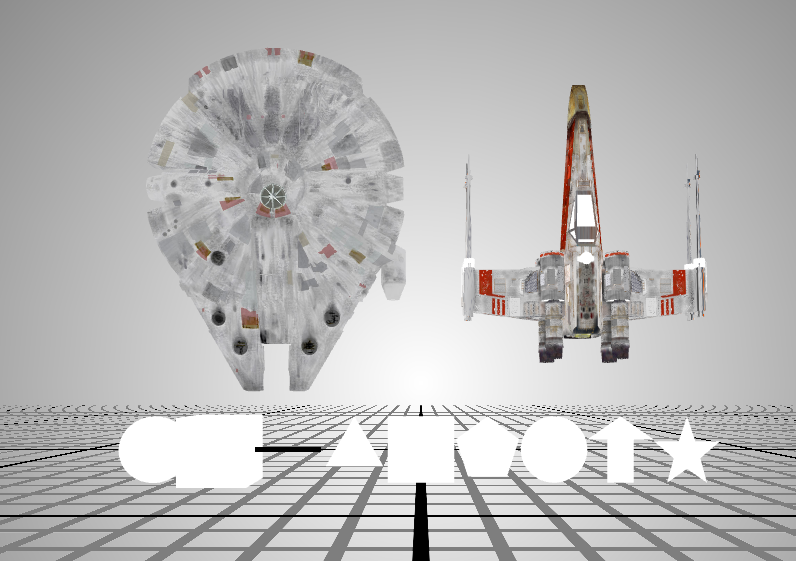
\includegraphics[scale=0.8]{fig/shapes.PNG}
	\caption{Formes 2D}
	\label{fig:primitives2D}
\end{figure}

\subsubsection{Forme vectorielle}
Les formes vectorielles offertes par cette application sont : une étoile et une flèche.
Sur la figure suivante, on peut voir tous les objets qu'il est possible de créer dans l'application, incluant les formes vectorielles.
\begin{figure}[H]
    \centering
	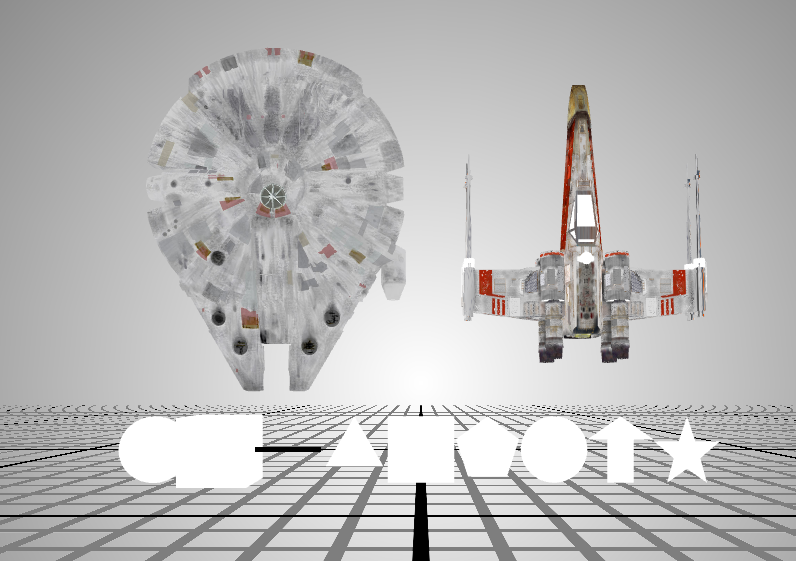
\includegraphics[scale=0.8]{fig/shapes.PNG}
	\caption{Formes 2D}
	\label{fig:formes2D}
\end{figure}

\subsubsection{Interface}
Nous avons décrit en grande majorité le fonctionnement de l’interface utilisateur et de ses éléments dans la section \ref{s:interactivité}.
Nous avons trois éléments d'interface graphique : l’inspecteur (pour modifier la position, la rotation, l’échelle de grandeur, la couleur et le parent des objets), le graphe de scène (voir tous les objets existant dans la scène ainsi que l’objet sélectionné) et l’interface de texture (offerte pour les objets 2D seulement, permettant de changer leur texture).
\begin{figure}[H]
    \centering
	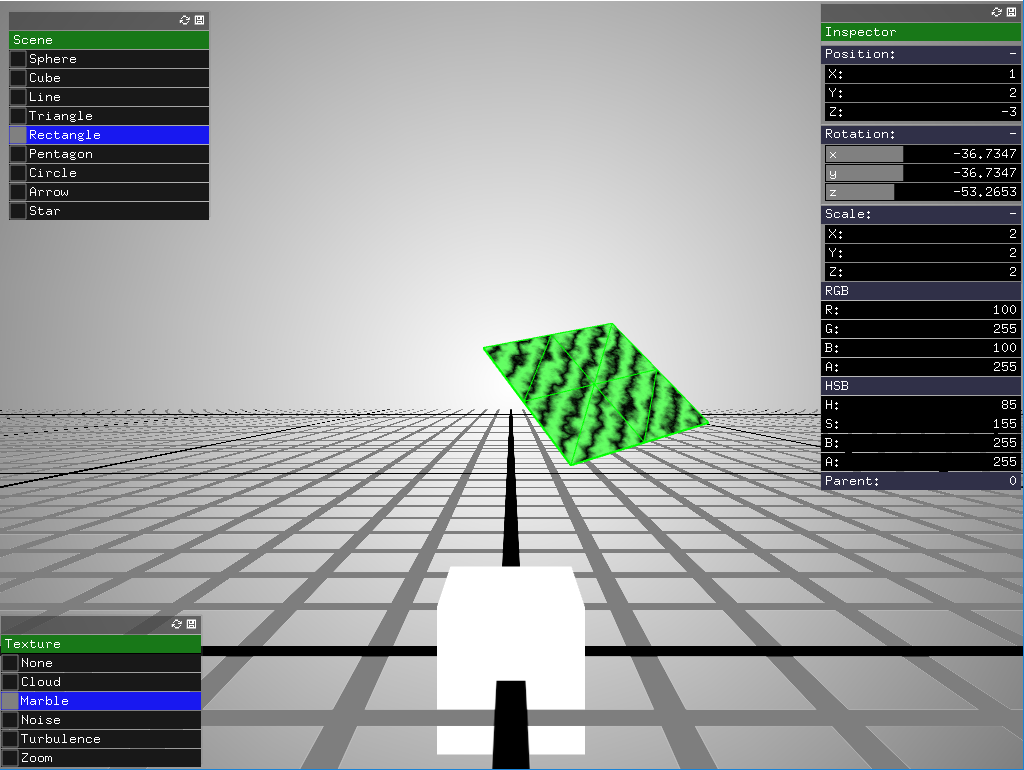
\includegraphics[scale=0.4]{fig/principale.PNG}
	\caption{Interface graphique}
	\label{fig:ui}
\end{figure}

\subsection{Transformation}
\subsubsection{Graphe de scène}
Le graphe de scène est une hiérarchie qui permet d’appliquer la transformation d’un parent sur ses objets enfants. On peut sélectionner un objet sur lequel on veut appliquer une transformation et il permet également de voir tous les éléments existant dans la scène. Pour plus d’information, voir \ref{fig:ui}.

\subsubsection{Transformations interactives}
L’interface utilisateur (le panneau Inspecteur) permet de façon interactive de changer la position, la rotation, la couleur, l’échelle de grandeur et le parent de l’objet sélectionné. Pour plus d’informations, se référer à \ref{fig:ui}.

\subsubsection{Historique des transformations}
\paragraph{} L'historique de transformation permet d'annuler et de récupérer une action provenant de l'utilisateur. Pour l'application, il est possible d'avoir l'historique du déplacement, de la rotation, de l'échelle et de la couleur pour chaque objet avec les touches \texttt{Ctrl+Z} et \texttt{Ctrl+Y}.
\paragraph{} L'état d'un objet \texttt{GameObject} est sauvegardé dans une classe \texttt{Command} à chacunes de ces actions. Le nombre de sauvegarde de commande est limité à 500. Cette commande est gérée par la classe \texttt{CommandHandler} qui s'occupe de sauvegarder les états courants (\texttt{CommandHandler::add()}), d'appliquer les changements d'état (\texttt{CommandHandler::undo()/redo()}) et d'ordonner les commandes dans deux \texttt{std::stack} dont une pour récupérer les commandes et une autre pour les annuler. Cette classe appartient à la classe \texttt{Scene} qui appelle la méthode de sauvegarde d'état à chaque fonction de modification d'un \texttt{GameObject}. Elle offre aussi les méthodes \texttt{Scene::undo()} et \texttt{Scene::redo()} pour que les événements puissent contrôler l'historique des transformations.

\subsection{Géométrie}
\subsubsection{Boîte de délimitation}
La boîte de délimitation permet de dessiner les arètes d’une boîte juste assez grande pour contenir les sommets d’un objet. Par contre, le Faucon Millénium et le « XWing » n’ont pas de boîte de délimitation car la position des sommets à l’intérieur du « mesh » est décalée par rapport au modèle 3D, ce qui dessinait la boîte très loin des objets eux-mêmes.
\begin{figure}[H]
    \centering
	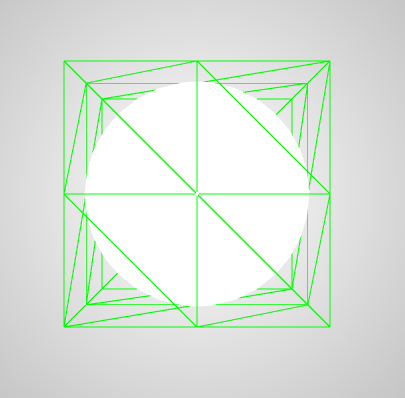
\includegraphics[scale=0.4]{fig/delimitation.PNG}
	\caption{Boîte de délimitation}
	\label{fig:box}
\end{figure}

\subsubsection{Primitives géométriques}
Les primitives géométriques offertes par cette application sont : un cube et une sphère.
Sur la figure suivante, on peut voir tous les objets qu'il est possible de créer dans l'application, incluant les primitives géométriques.
\begin{figure}[H]
    \centering
	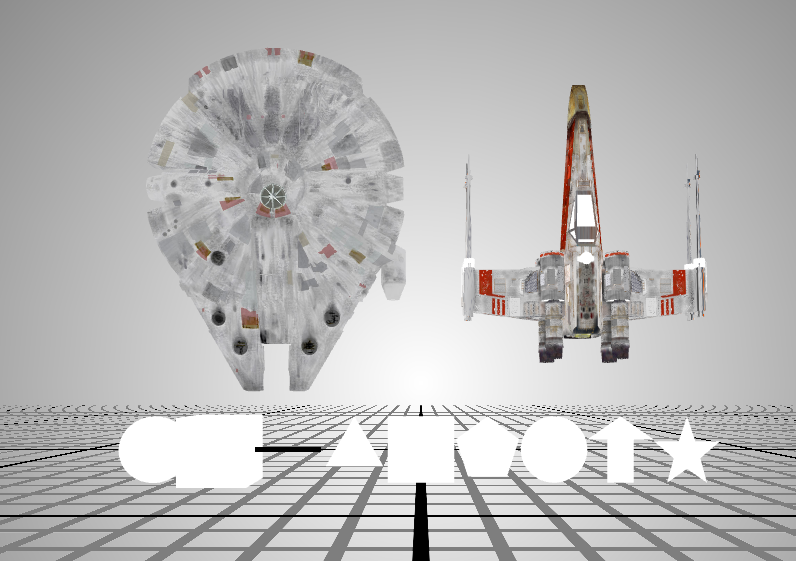
\includegraphics[scale=0.8]{fig/shapes.PNG}
	\caption{Primitives géométriques}
	\label{fig:primitivesgeo}
\end{figure}

\subsubsection{Modèle 3D}
Les modèles 3D offerts par cette application sont : le \textit{Faucon Millenium} et le \textit{X-Wing Fighter}.
Sur la figure suivante, on peut voir tous les objets qu'il est possible de créer dans l'application, incluant les modèles 3D.
\begin{figure}[H]
    \centering
	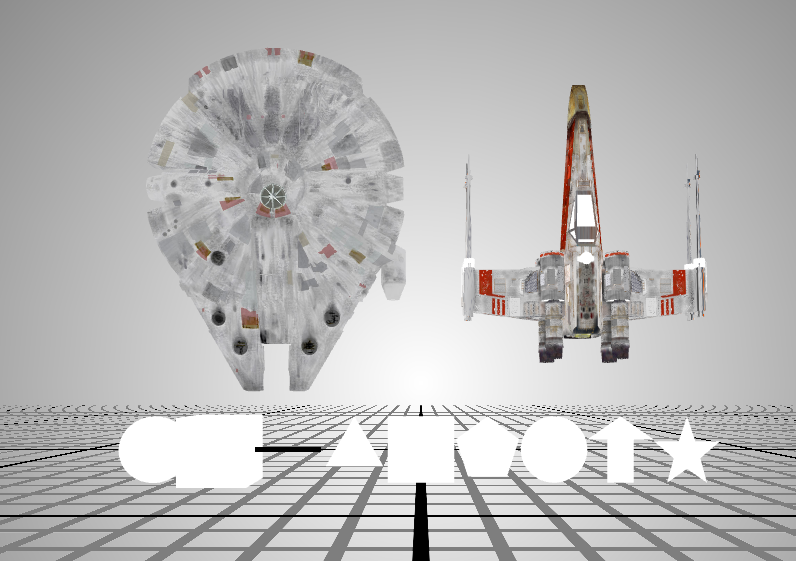
\includegraphics[scale=0.8]{fig/shapes.PNG}
	\caption{Modèles 3D}
	\label{fig:modeles3D}
\end{figure}

\subsection{Texture}
\subsubsection{Mapping}
Les modèles 3D du \textit{Faucon Millenium} ainsi que du \textit{X-Wing Fighter} sont texturés avec des coordonnées de mapping contenues dans leur fichier .OBJ respectif.
Le add$-$ons \textit{ofxAssimpModel} permet de charger ces modèles et s'occupe de créer les coordonnées de textures correspondant à chaque sommet.
Sur la figure suivante, on peut voir les deux modèles avec leur texture appliquée adéquatement.
\begin{figure}[H]
    \centering
	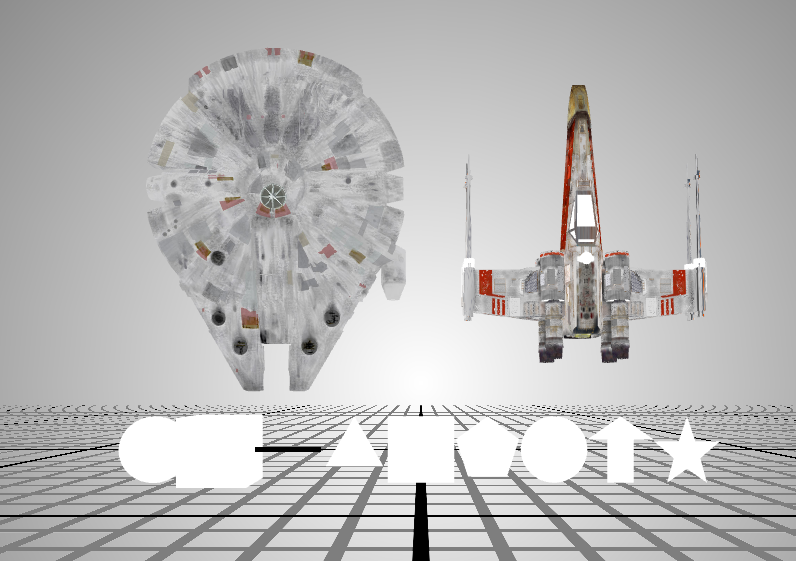
\includegraphics[scale=0.4]{fig/shapes.PNG}
	\caption{Modèles 3D texturés}
	\label{fig:mapping}
\end{figure}

Chaque forme 2D qu'il est possible de créer (ligne, rectangle, triangle, cercle, pentagone, flèche et étoile) possède des coordonnées de texture permettant de leur associer les textures procédurales.
Par exemple, la figure suivante montre l'étoile texturée.
\begin{figure}[H]
    \centering
	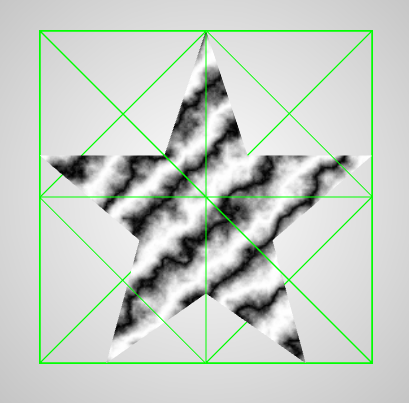
\includegraphics[scale=0.4]{fig/star.PNG}
	\caption{Étoile texturée}
	\label{fig:mapping2}
\end{figure}



\subsubsection{Texture procédurale}
\paragraph{} Les textures procédurales proviennent d'un patron de base sur lequel est appliqué des algorithmes. Les patrons de bases utilisés sont le bruit de perlin, le patron en sinus et le patron en cercle.
\paragraph{} Il est possible de générer une texture procédurale imitant l'effet nuage avec le bruit de perlin, une interpolation linéaire, un algorithme de turbulence et une modification les paramètres HSL. L'effet marbre est généré par le patron en sinus sur lequel on applique un algorithme de turbulence. L'effet bois est généré par le patron en cercle sur lequel on applique un algorithme de turbulence ainsi qu'un filtre de couleur bois (orangé / brun).
\begin{figure}[H]
\centering
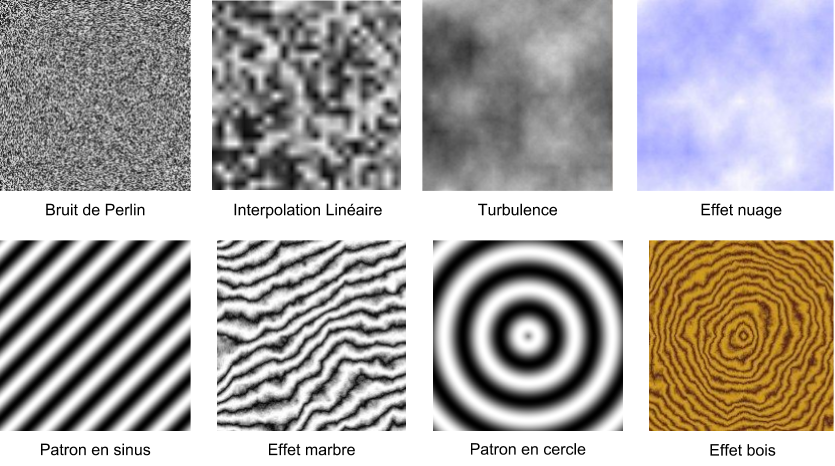
\includegraphics[width=\textwidth]{img/infog-image-procedural-texture.png}
\caption{Textures procédurales}\label{fig-procedural-texture}
\end{figure}
\paragraph{} Au niveau de l'application, une classe \texttt{texelFactory} s'occupe de générer toutes les textures procédurales présentées plus-haut (\ref{fig-procedural-texture}).  Chaque textue est interfacée par une méthode permettant de transformer un buffer \texttt{ofPixels} avec des paramètres (puissance de la turbulence par exemple) qui seront utilisées par les algorithmes correspondants (réf. \ref{src-procedural-texture}). Par la suite, ce buffer est appliqué sur le \texttt{GameObject} qui possède un \texttt{ofTexture} et un \texttt{ofMesh} propre. Aussi, lors de la création du \texttt{ofMesh}, il est nécessaire de cartographier la texture sur la forme avec la méthode \texttt{ofMesh::addTextCoord} et \texttt{ofTexture::getCoordFromPercent}.

%%%%%%%%%%%%%%      TP2      %%%%%%%%%%%%
% >> CAMÉRA
\subsection{Caméra}
\subsubsection{xxx}

% >> ILLUMINATION
\subsection{Illumination}
\subsubsection{Modèle d'illumination}
\label{s:illumination}
Les modèles d'iilumination choisi sont \textit{remplissage de couleur}, \textit{lambert}, \textit{gouraud}, \textit{phong} et \textit{blinn-phong}. Dans la scène, il est possible de passer d'un modèle d'illumination à l'autre grâce à la touche \textbf{'q'}. Ces modèles sont appliqués aux primitives avec des \textit{shaders} qui se trouvent dans le dossier \textit{bin/data/shadersRender}. Il est représenté par la classe \texttt{Render} qui se trouve à l'intérieur de la classe \texttt{Scene}. Le \textit{shader} est appliqué sur tous les \texttt{GameObject} lors de l'appel de la fonction \texttt{Scene::draw()}.

\begin{figure}[H]
    \centering
	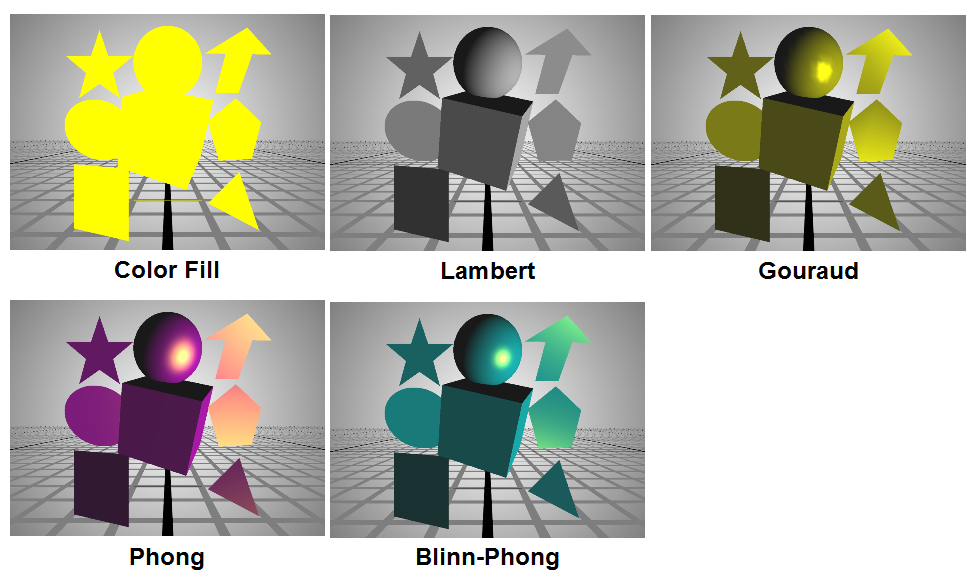
\includegraphics[scale=0.6]{img/infog-image-modele-illumination.png}
	\caption{Rendu des modèles d'illumination}
	\label{fig:illuminationmodel}
\end{figure}

% >> LANCER DE RAYON
\subsection{Lancer de rayon}
\subsubsection{xxx}

% >> TOPOLOGIE
\subsection{Lancer de rayon}
\subsubsection{xxx}

% >> TECHNIQUE DE RENDU
\subsection{Techniques de rendu}
\subsubsection{Effet en pleine fenêtre}
\label{s:effect}
Les effets en pleine fenêtre sont gérés par la classe \texttt{fboRender}. Cette classe permet d'appliquer 3 types d'effet visuel dont un effet \textbf{flou gaussien}, un effet \textbf{noir et blanc} et un effet \textbf{sépia}. Il est possible de passer d'un effet à un autre avec la touche \textbf{'e'} lorsque le logiciel est lancé. \\

Chaque effet est géré par son propre shader qui se trouve dans le dossier \texttt{bin/data/shaders} qui contient les fichiers \textit{Vertex Shader} et \textit{Fragment Shader}. Le principe est de dessiner la scène dans un élément \texttt{ofFbo} pour rastériser le plan image afin d'appliquer par la suite le \texttt{shader} approprié. Enfin, on dessine l'objet \texttt{ofFbo} pour afficher le résultat à l'écran.

\begin{figure}[H]
    \centering
	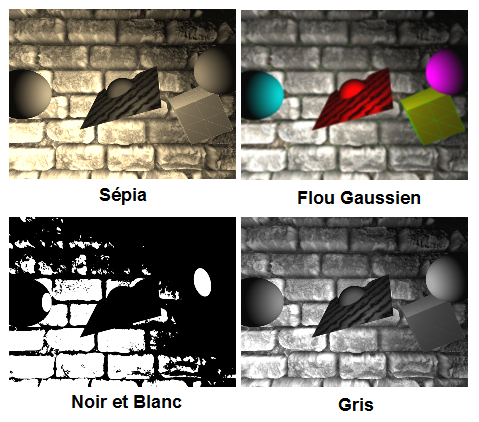
\includegraphics[scale=0.8]{img/infog-image-effet-plein-ecran.png}
	\caption{Application des effets sur la scène en cours.}
	\label{fig:effects}
\end{figure}


\subsubsection{Effet de relief}
\label{s:relief}
La technique d'effet en relief choisi est un mélange entre du \textit{normal mapping} et du \textit{bump mapping} sur un mur de brique de pierre. Cet effet de relief est représenté par la classe \texttt{planeRelief} qui contient le \texttt{ofShader} qui applique les fichiers \textit{normalMap.frag/vert}, des \texttt{ofImage} pour charger la texture, la texture \textit{bump mapping} et la texture \textit{normal mapping}. Le \textit{shader} assigne les textures, la profondeur maximum et la position de la lumière qui sont ensuite appliqué sur la primitive \texttt{ofPlanePrimitive}.

\begin{figure}[H]
    \centering
	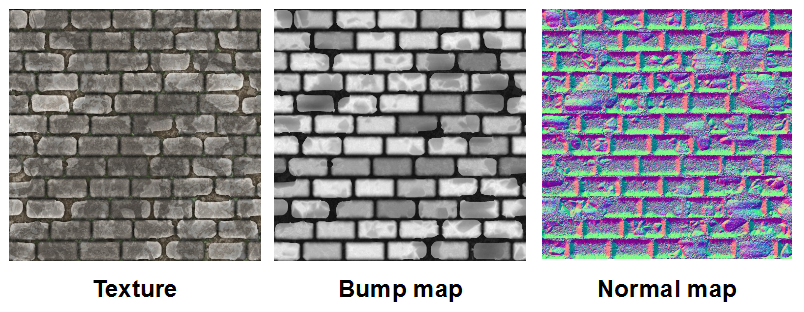
\includegraphics[scale=0.8]{img/infog-image-mur-pierre.png}
	\caption{Fichiers textures du mur de pierre.}
	\label{fig:wallfiles}
\end{figure}

La texture \textbf{Bump Map} sert à ajouter de la profondeur en repositionnant chaque point de la surface en fonction de la valeur de ce point sur la texture \textbf{Bump Map} avec une profondeur fixée par une variable, ce qui donne l'\textbf{Effet Bump Map} ci-dessous. \\

La texture \textbf{Normal Map} sert à ajouter un effet relief grâce à la position de la lumière ambiante par rapport à la normal de la surface qui est représenté par la valeur est canaux RGB de la texture \textbf{Normal Map}. L'ombrage de chaque pixel est calculé par la suite grâce à la position de la lumière et de la normal à ce point, ce qui donne l'\textbf{Effet Normal map} ci-dessous.

\begin{figure}[H]
    \centering
	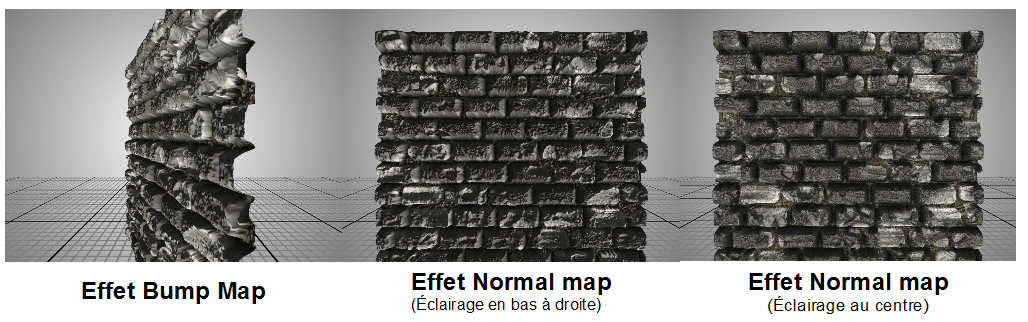
\includegraphics[scale=0.62]{img/infog-image-rendu-mur-pierre.png}
	\caption{Rendu des effets de relief sur le mur de pierre}
	\label{fig:wallnormalbumprender}
\end{figure}

\subsubsection{Style libre}

Le style libre est l'effet visuel cartoon en temps réel qui fait partie de la classe \texttt{fboRender}. Il s'agit d'une combinaison d'effet gérée par des \textit{shaders} qui permet d'arriver à ce résultat. \\

Trois traitements principaux sont identifiés :
\begin{itemize}
\item \textbf{Baisse de la résolution des couleurs originales}\\
Cette baisse de résolution se fait par le \textit{shaders/colorbits.frag} qui va la réduire à 4 valeurs pour chaque canal RGB.
\item \textbf{Détection des lignes de contours}\\
Cette phase applique deux traitements à l'image d'origine dont l'application du \textit{shaders/blackwhite.frag} pour obtenir l'image en noire et blanche suivi d'un détecteur de contours (Filtre de Sobel) avec \textit{shaders/edgesobel.frag}.
\item \textbf{Combinaison des deux images}\\
Il s'agit d'une simple multiplication entre la texture avec détection de contours et la texture à basse résolution grâce à au \textit{shaders/multiple.frag}. \\
\end{itemize}

Chacune des étapes se fait par le biais d'un objet \texttt{ofFbo} pour chaque application de \textit{shader}.


\begin{figure}[H]
    \centering
	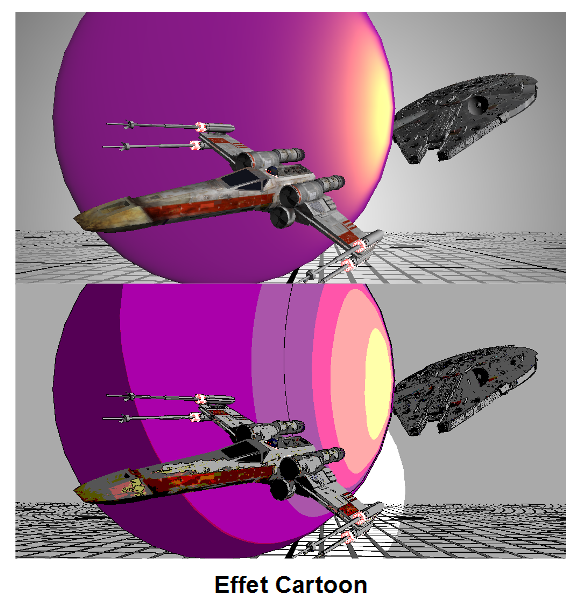
\includegraphics[scale=1]{img/infog-image-effet-cartoon.png}
	\caption{Rendu de l'effet cartoon sur une scène}
	\label{fig:cartooneffect}
\end{figure}